\documentclass[sigconf, nonacm]{acmart}


\usepackage{draftwatermark}
\SetWatermarkText{AI-Generated}
\SetWatermarkScale{0.5}
\SetWatermarkColor[gray]{0.6}
\AtBeginDocument{\providecommand\BibTeX{{Bib\TeX}}}

\copyrightyear{2025}
\acmYear{2025}
\setcopyright{none}
\acmConference[arXiv preprint]{arXiv preprint}{2025}{}
\acmBooktitle{}
\acmDOI{}
\acmISBN{}
\settopmatter{printacmref=false}         
\renewcommand\footnotetextcopyrightpermission[1]{} 

\usepackage{multirow}
\usepackage{enumitem}
\usepackage[skip=2pt]{caption}
\usepackage{bm}
\graphicspath{{figures/}}


\begin{document}
\title{FoodLogAthl-218: Constructing a Real-World Food Image Dataset\\ Using Dietary Management Applications}

\author{Anonymous Author}

\begin{abstract}
Food recognition models for dietary logging are usually trained and evaluated on web-crawled images that are attractive, curated for a predefined label set, class-balanced, and mostly show a single dish, whereas photos taken for personal meal logging are casual, heavily imbalanced, temporally ordered, and often contain several dishes. This mismatch makes it hard to judge how well current systems would work in a real logging application. We introduce FoodLogAthl-218, a benchmark built bottom-up from meal photos that users submitted to the dietary management application FoodLog Athl and labeled afterwards: the raw logs (11,460 images, 61,414 bounding boxes, 5,889 raw labels) are filtered by class size, CLIP-based outlier detection and manual review, and their labels are consolidated with GPT-4o-assisted grouping and human adjudication, yielding 6,925 images, 14,349 dish bounding boxes, 218 classes and 513 users, with anonymized user IDs, timestamps and meal context. We define three tasks: closed-set dish classification on crops, continual user-aware adaptation along the time axis, and menu-aware classification of dishes in multi-dish images. Ten large multimodal models and CLIP-style encoders are evaluated: the best Top-1 recall is 0.424 (GPT-4o), the best Top-5 recall is 0.600 (CLIP ViT-L/14), and rankings change with the metric. Compared with UEC-Food 256, the dataset shows larger intra-class spread and weaker cluster separation in three feature spaces. A zero-shot model deteriorates over time, while fine-tuning on accumulated logs raises accuracy from roughly 0.2 to roughly 0.5; a single heavy logger benefits strongly from user-specific adaptation. Adding whole-image descriptions improves precision and F1 but lowers recall. We also state what the benchmark does not measure, including its single-application source and the lack of inter-annotator agreement.
\end{abstract}

\maketitle

\section{Introduction}
Dietary logging applications let people record what they eat by photographing meals, and automatic food recognition is the component that makes this convenient~\cite{aizawa2015foodlog,nakamoto2022foodlog,DBLP:journals/corr/abs-1808-07202}. Progress in this area is measured on food image datasets such as Food-101 and UEC-Food 256~\cite{bossard2014food,kawano2015automatic}, which are typically assembled by choosing a list of dish categories and then collecting images for them, usually from the web. The resulting data differ from what a logging application sees in several ways (Figure~\ref{fig:comparison}): categories are roughly balanced or curated, photos are chosen to be appealing for public sharing, samples are independent of each other, and an image usually shows a single dish. Personal meal photos instead follow the long-tailed frequency of what people actually eat, are taken casually for private use, form a personal time series, and frequently show a whole meal with several dishes. Consequently, results on web-sourced benchmarks may say little about performance in deployment, and they cannot probe questions that matter for logging, such as whether a model improves as it accumulates a user's records, or whether the other dishes in the same meal help.

\begin{figure*}[t]
  \centering
  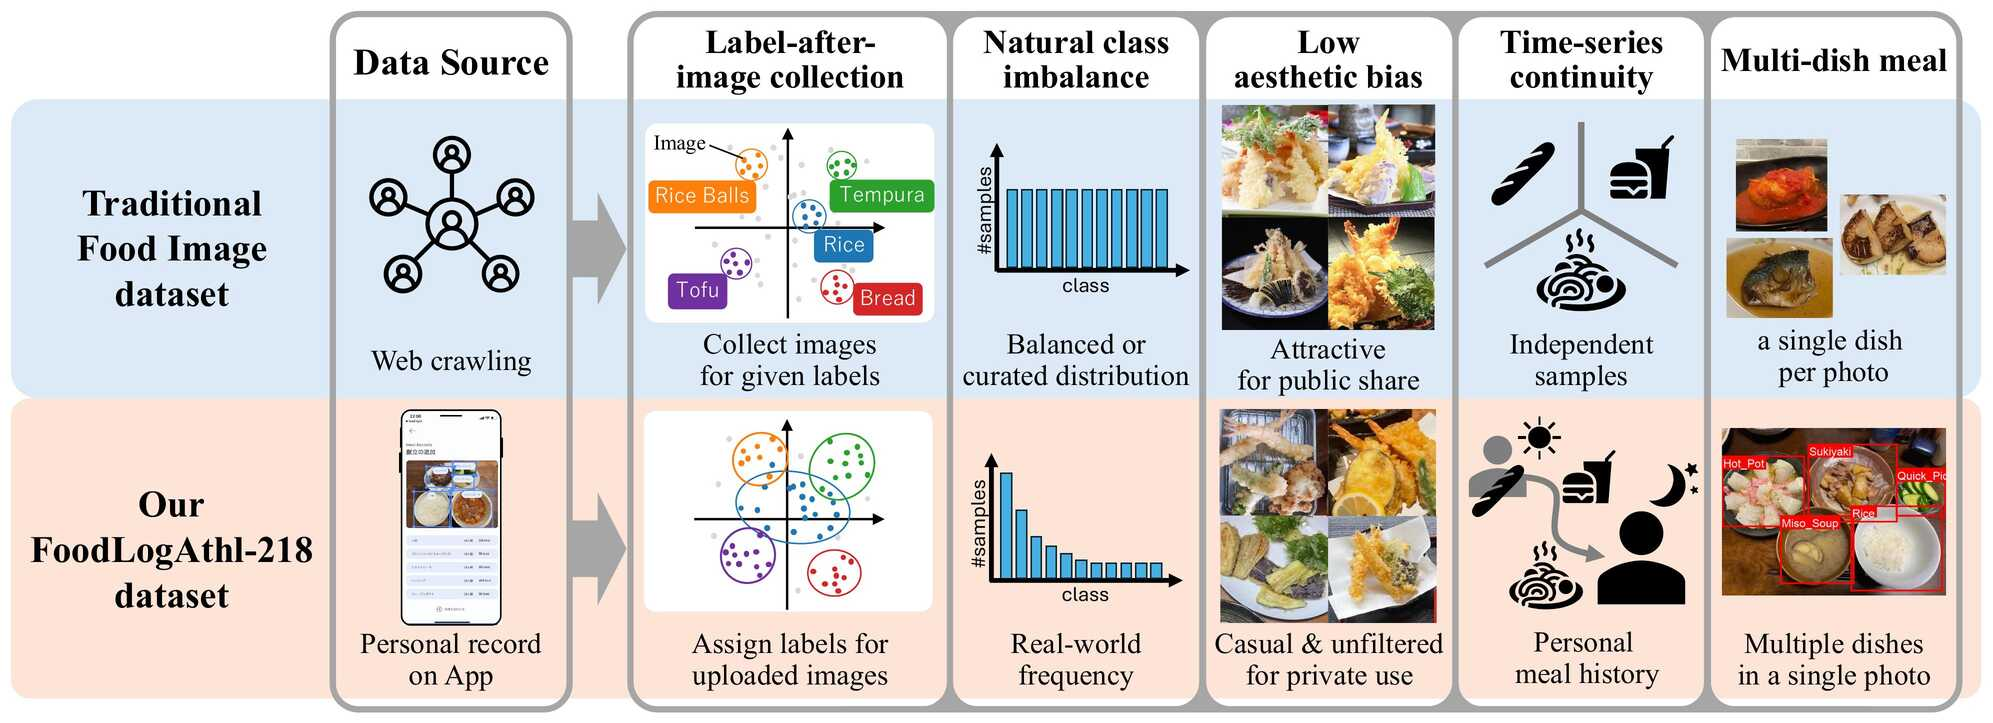
\includegraphics[width=0.85\textwidth]{distribution_5.jpg}
  \caption{Comparison between traditional web-sourced food image datasets and FoodLogAthl-218 along data source, label assignment, class distribution, image style, temporal structure and number of dishes per photo.}
  \label{fig:comparison}
\end{figure*}

We therefore present \emph{FoodLogAthl-218}, a benchmark constructed from the records of the FoodLog Athl application~\cite{nakamoto2022foodlog}. Its design follows a ``label-after-image-collection'' principle: images are taken as users uploaded them, and the label space is derived afterwards by cleaning and merging the labels users and the application attached to them, rather than fixed beforehand. This keeps natural class imbalance, casual imaging conditions, multi-dish meals and temporal continuity, at the price of some residual label noise and a skewed, application-specific population, which we document. The benchmark comprises 6,925 images, 14,349 dish bounding boxes, 218 classes and 513 users.

On this data we define three tasks (Figure~\ref{fig:tasks}): (1) closed-set classification of dish crops; (2) continual user-aware adaptation, in which a model is repeatedly updated with the logs accumulated so far and evaluated on the following weeks; and (3) menu-aware classification, in which a description of the whole meal is available when classifying one dish. We evaluate ten representative systems, large multimodal models (LMMs) through \texttt{lmms-eval}~\cite{lmms_eval2024,zhang2024lmmsevalrealitycheckevaluation} and CLIP-style encoders~\cite{CLIP,sun2023eva}, and run fine-tuning experiments on Task~2.

\paragraph{Main findings.} The closed-set task is hard (best Top-1 recall 0.424, best Top-5 recall 0.600, with different systems best under different metrics); the dataset is more spread and less separable than UEC-Food 256 in all three feature spaces tested; zero-shot accuracy does not improve over time while fine-tuning on accumulated logs lifts it to roughly 0.5; and whole-meal descriptions trade recall for precision.

\paragraph{Contributions.}
\begin{itemize}[leftmargin=*,topsep=2pt,itemsep=1pt]
  \item A real-world food image benchmark from a dietary management application, with natural class imbalance, multi-dish meals and timestamps, collected with ethics approval and informed consent and screened for personal information.
  \item A documented, mixed automated--human curation pipeline (class-size filtering, CLIP outlier detection, manual review, GPT-4o-assisted label grouping with human adjudication) with per-step statistics.
  \item Three tasks and metrics that correspond to practical needs of dietary logging: closed-set, continual user-aware, and menu-aware classification.
  \item Baseline results for LMMs and CLIP-style models, a distributional comparison with UEC-Food 256, and analyses of temporal adaptation, personalization and meal context, together with an explicit statement of limitations.
\end{itemize}

\begin{figure}[t]
  \centering
  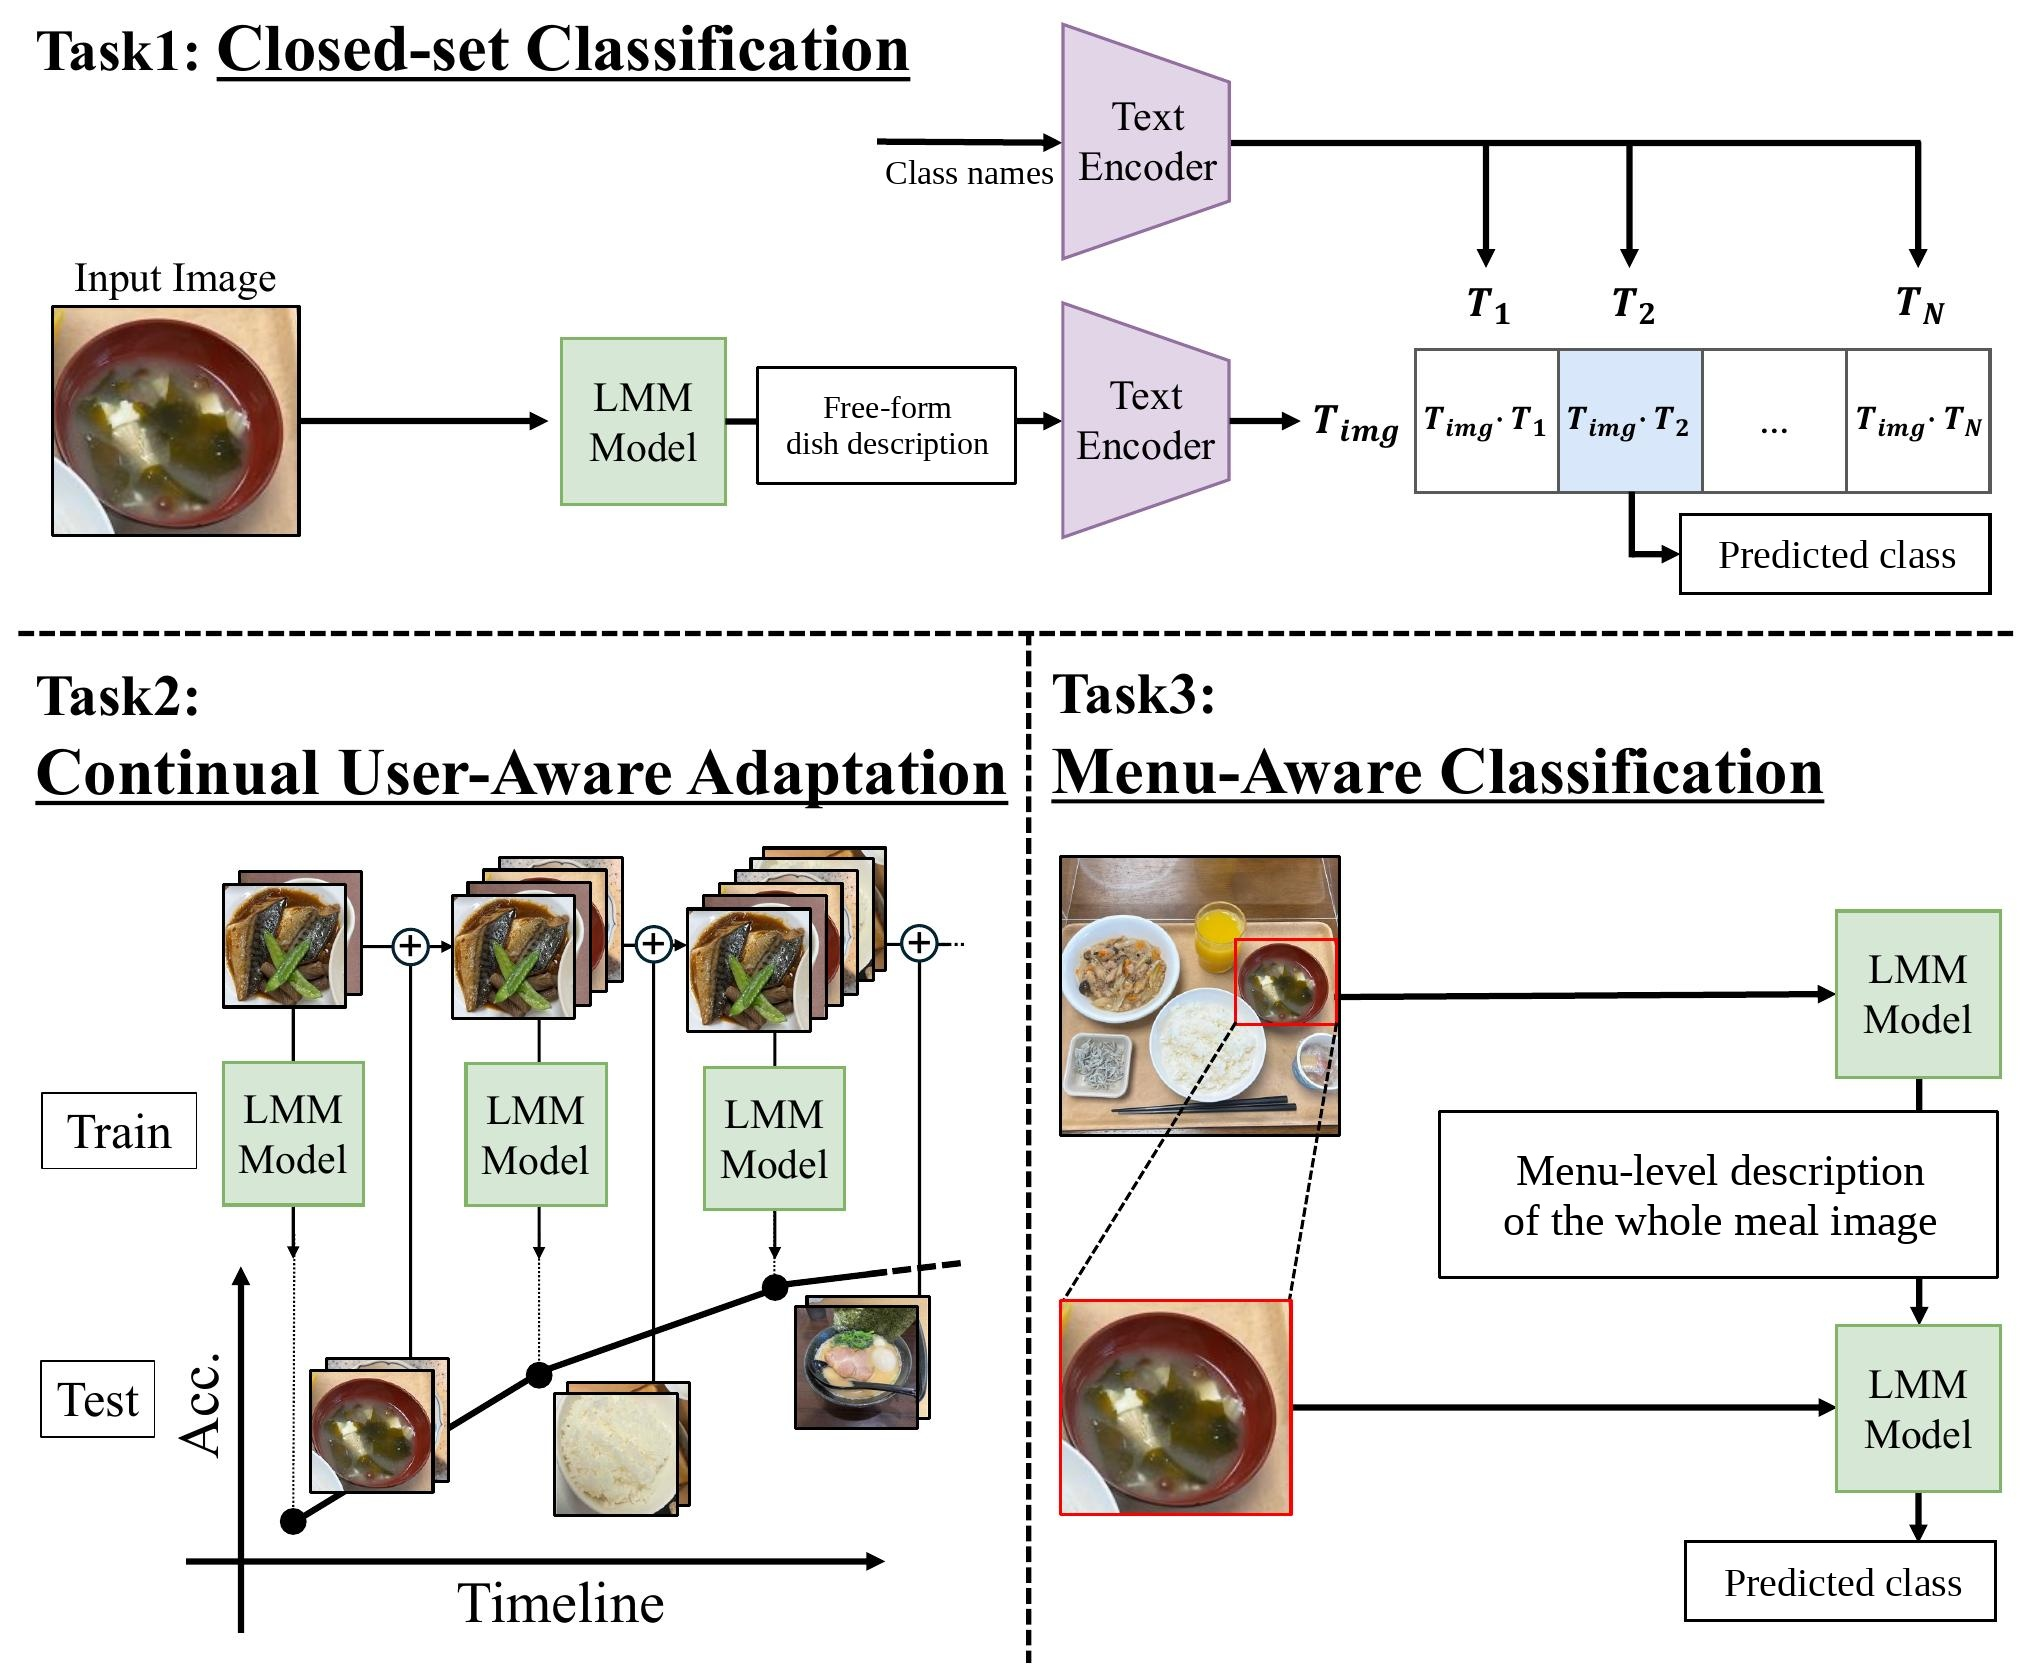
\includegraphics[width=0.7\columnwidth]{ACM_task.jpg}
  \caption{Overview of the three benchmark tasks: closed-set classification of dish crops (LMM output embedded and matched to class names), continual user-aware adaptation along the timeline, and menu-aware classification using a description of the full meal image.}
  \label{fig:tasks}
\end{figure}

\section{Related Works}
\paragraph{Food image datasets.} Early food datasets such as PFID, UEC-Food and Food-101 established image-level and dish-level recognition~\cite{chen2009pfid,joutou2009food,kawano2015automatic,bossard2014food}, followed by larger and more varied collections, including UPMC Food-101, Vegfru, FoodAI-756 and Food2K~\cite{wang2015recipe,hou2017vegfru,sahoo2019foodai,min2023large}, and by recipe-, ingredient- and nutrition-oriented resources such as Recipe1M+ and Nutrition5k~\cite{marin2019learning,thames2021nutrition5k}. Table~\ref{Food image dataset table} summarizes the main image classification datasets. Almost all draw on web search or web platforms, or on participants asked to photograph food (UNICT-FD1200~\cite{farinella2016retrieval}), and fix the categories before collecting images. FoodLogAthl-218 is, to our knowledge among the datasets in this table, the only one drawn from a dietary management application; it is smaller than the web-scale collections and covers fewer classes than several of them, so we position it as a realism-oriented evaluation set rather than a training corpus of comparable scale.

\paragraph{Food recognition in logging applications and personalization.} Food logging systems that combine recognition with user records, including FoodLog and FoodLog Athl~\cite{aizawa2015foodlog,nakamoto2022foodlog}, have motivated work on exploiting personal dietary tendencies and personalized classifiers~\cite{Aizawa2013FoodBalance,flg469}. Task~2 is designed to let such user-level adaptation be compared on timestamped, user-attributed real logs.

\paragraph{Foundation models for food and their evaluation.} Contrastive vision--language models~\cite{CLIP,sun2023eva} and LMMs~\cite{liu2024visual,liu2024improved,bai2023qwen,achiam2023gpt} are now applied to food understanding, for example in food-specific assistants and Japanese recipe generation~\cite{yin2023foodlmm,Imajuku2025FoodMLLM}, and benchmarks for them increasingly include food-related questions, such as multicultural dish question answering~\cite{winata2024worldcuisines} and food captioning~\cite{ma2023food}. Evaluation toolkits such as \texttt{lmms-eval}~\cite{lmms_eval2024,zhang2024lmmsevalrealitycheckevaluation} make it possible to compare such models under one protocol, which we use. Our benchmark adds a classification setting with real-world imbalance, user identity, and time, on which both CLIP-style and generative models can be assessed.

\begin{table*}[thb]
\centering
\caption{Food image classification datasets. \#samples is the sample count reported for each dataset; for FoodLogAthl-218 it counts dish bounding boxes (14,349 boxes in 6,925 images, since one image can hold several dishes). Web-sourced data are marked in bold.}
\begin{tabular}{@{}rllrrll@{}}
\toprule
Year & Dataset & Cuisine & \#classes & \#samples & Data source \\
\midrule
2009 & PFID~\cite{chen2009pfid} & Western & 101 & 4,545 & Fast food chains \\
2014 & UEC-Food 256~\cite{kawano2015automatic} & International & 256 & 25,088 & \textbf{Web} + original database \\
2014 & Food-101~\cite{bossard2014food} & Western & 101 & 101,000 & \textbf{Web} (foodspotting.com) \\
2015 & UPMC Food-101~\cite{wang2015recipe} & Western & 101 & 90,840 & \textbf{Web} (Google~\cite{google}) \\
2016 & UNICT-FD1200~\cite{farinella2016retrieval} & International & 1,200 & 4,754 & Experiment participants \\
2017 & Vegfru~\cite{hou2017vegfru} & Vegetables, fruits & 25/292\textsuperscript{*} & 160,000 & \textbf{Web} (Google, ImageNet~\cite{imagenet}, etc.) \\
2019 & FoodAI-756~\cite{sahoo2019foodai} & International & 152/756\textsuperscript{*} & 400,000 & \textbf{Web} (Google, Bing, etc.) \\
2021 & Food2K~\cite{min2023large} & International & 2,000 & 1,036,564 & \textbf{Web} (Meituan~\cite{meituan}) \\
2023 & Food-500 Cap~\cite{ma2023food} & International & 494 & 24,700 & \textbf{Web} (Google, Bing) \\
\midrule
2025 & FoodLogAthl-218 (ours) & International & 218 & 14,349 & Dietary management app \\
\bottomrule
\end{tabular}

\smallskip
\raggedright\footnotesize\textsuperscript{*}Hierarchically structured dataset; $n$/$m$ means $m$ classes grouped into $n$ higher-level classes.
\label{Food image dataset table}
\end{table*}


\section{FoodLogAthl-218 Dataset}
\subsection{Source and collection}
FoodLog Athl is a dietary management application in which users photograph meals and the application proposes dish regions and names, drawn from a database of about 140K food items; users can correct names and add portion sizes~\cite{nakamoto2022foodlog}. We use records from May 2023 to October 2024: initially 11,460 images with 61,414 bounding boxes and 5,889 distinct raw labels from 632 users. Each record carries an anonymized user ID, date and time, dish names, portion size and the initial detections. The study has ethics approval and informed consent, and personal information was removed in two manual stages. Images are treated as atomic units, so multi-dish meals are never split across the dataset.

\subsection{Curation pipeline}
Table~\ref{data cleaning steps table} lists the steps and their effect. (1) Records without an image, and (2) images without a bounding box, are dropped (11,285 images remain). (3) Classes with fewer than ten samples are removed (1,180 classes remain), since such classes cannot be evaluated or learned meaningfully. (4) Samples whose CLIP~\cite{CLIP} ViT-B/16 embedding lies more than 1.5 standard deviations from its class centroid are flagged and removed (7,537 images). (5) Reviewers manually fix or remove invalid boxes and labels (Figure~\ref{fig:errors}); whenever one dish of an image is removed, the whole image is removed (``all-or-none'') so that remaining meals stay complete, leaving 6,925 images, 14,349 bounding boxes and 513 users. (6) Finally, GPT-4o groups synonymous or near-duplicate labels into clusters, and human reviewers refine and adjudicate them, merging the 1,180 classes into 218 final classes. The steps operate on the user's own labels, so the final label space is a product of what people log, not of a designer's taxonomy.

\begin{table*}[tb]
  \centering
  \caption{Data filtering and curation pipeline: counts after each step, with the change from the previous step. Steps~1--2 remove log records without a usable image or bounding box, step~3 drops classes with fewer than 10 samples, step~4 flags crops more than 1.5 SD from their class centroid in CLIP ViT-B/16 feature space, step~5 is manual review (an image is removed entirely if any of its dishes is invalid, so meal composition is preserved), and step~6 consolidates synonymous labels (GPT-4o grouping followed by manual refinement). Counts are of images, dish bounding boxes (bboxes) and distinct classes.}
  \begin{tabular}{@{}cl rr rr rr@{}}
    \toprule
    Step & Operation & \multicolumn{2}{c}{\#images} & \multicolumn{2}{c}{\#bboxes} & \multicolumn{2}{c}{\#classes} \\
    & & count & $\Delta$ & count & $\Delta$ & count & $\Delta$ \\
    \midrule
    0 & Raw data & 11,460 &  & 61,414 &  & 5,889 &  \\
    1 & Remove samples w/o image & 11,460 & 0 & 26,646 & $-$34,768 & 3,167 & $-$2,722 \\
    2 & Remove samples w/o bounding box & 11,285 & $-$175 & 26,065 & $-$581 & 3,071 & $-$96 \\
    3 & Remove classes w/ $<$10 samples & 9,121 & $-$2,164 & 21,944 & $-$4,121 & 1,180 & $-$1,891 \\
    4 & Remove outliers based on image features & 7,537 & $-$1,584 & 17,513 & $-$4,431 & 1,180 & 0 \\
    5 & Manual review, remove invalid images & 6,925 & $-$612 & 14,349 & $-$3,164 & 1,180 & 0 \\
    6 & Merge similar classes, clean labels & 6,925 & 0 & 14,349 & 0 & 218 & $-$962 \\
    \bottomrule
  \end{tabular}
  \label{data cleaning steps table}
\end{table*}


\begin{figure*}[t]
  \centering
  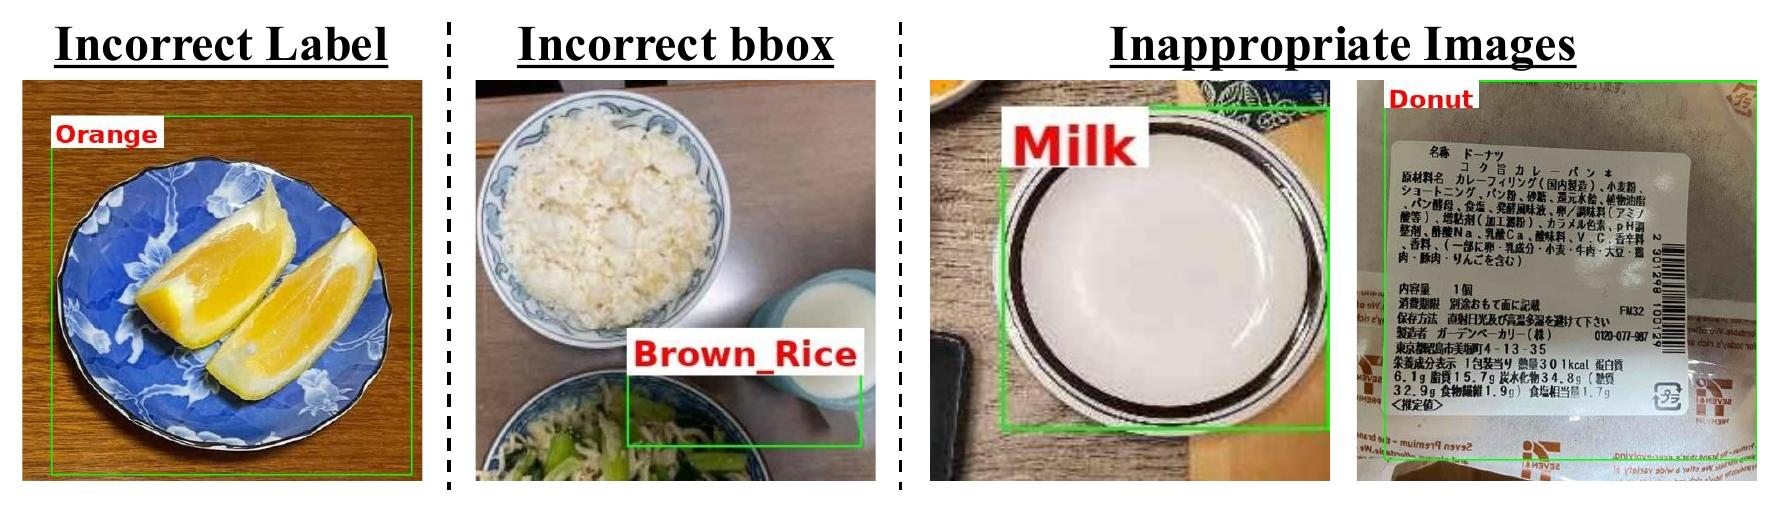
\includegraphics[width=0.7\textwidth]{error_example.jpg}
  \caption{Examples of erroneous data found in the raw logs and removed or corrected in manual review: incorrect labels, incorrect bounding boxes, and inappropriate images.}
  \label{fig:errors}
\end{figure*}

\subsection{Dataset characteristics}
Figure~\ref{fig:hist} shows the number of images per class on a logarithmic axis. By construction every class has at least ten samples, many classes are near this minimum, and a few have on the order of $10^3$ images, so the distribution is long-tailed, as in real logging. Typical images are casual photographs with cluttered backgrounds, packaged food and several dishes per image (the examples in Figures~\ref{fig:errors} and~\ref{fig:desc} are representative).  The benchmark includes users with long logging histories, which Task~2 uses to study personalization; we do not report per-user image counts here.

\begin{figure}[t]
  \centering
  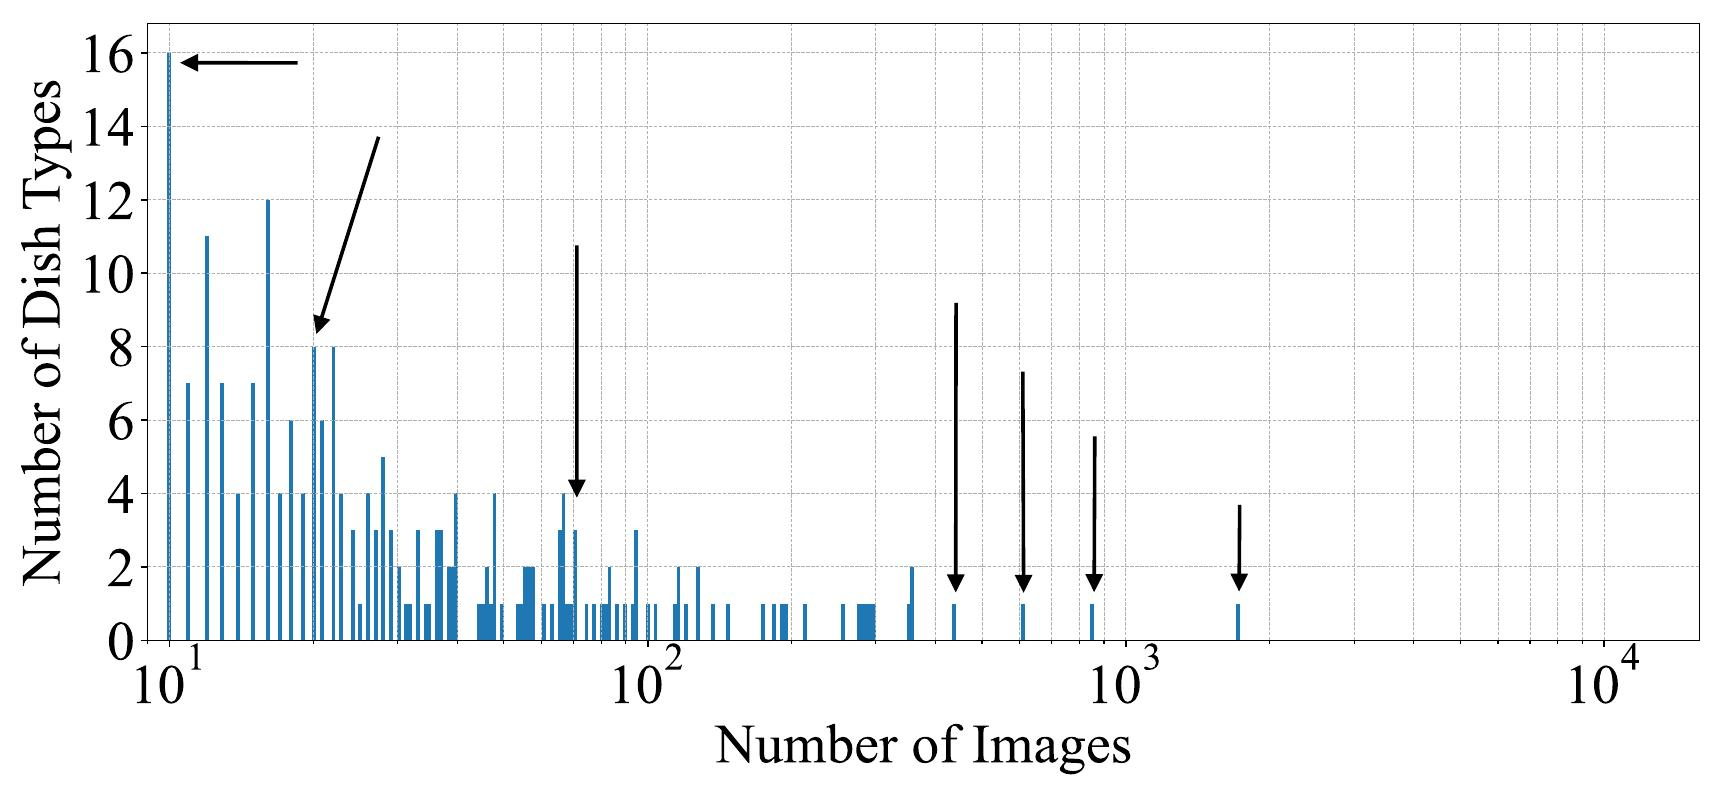
\includegraphics[width=0.9\columnwidth]{histogram_linear_pdf.jpg}
  \caption{Number of dish types (classes) by number of images per class (logarithmic horizontal axis, linear vertical axis); arrows mark illustrative classes shown in the original figure.}
  \label{fig:hist}
\end{figure}

\subsection{Validation: diversity relative to a web-sourced benchmark}
To test whether the dataset is harder to separate than a conventional benchmark, we compare feature-space statistics with UEC-Food 256~\cite{kawano2015automatic}, using three image encoders (CLIP~\cite{CLIP}, EVA-CLIP~\cite{sun2023eva}, Swin Transformer~\cite{liu2021swin}). We report the trace of the feature covariance (larger means more spread), the silhouette score~\cite{rousseeuw1987silhouettes}, the Davies--Bouldin index~\cite{davies1979cluster} and the Calinski--Harabasz index~\cite{calinski1974dendrite}, using class labels as clusters. Table~\ref{table:diversity_metrics_comparison} shows that FoodLogAthl-218 has larger trace, lower silhouette, higher Davies--Bouldin and lower Calinski--Harabasz values than UEC-Food 256 in every one of the three feature spaces, i.e., classes are more spread out and overlap more. For example, the CLIP trace is 81.70 versus 71.21 and the CLIP silhouette $-0.021$ versus $0.033$. All twelve comparisons point the same way, but the metrics are descriptive: they are computed on different class inventories (218 versus 256 classes) and sample sizes, they are not comparable across encoders, and they do not by themselves establish difficulty. The classification results below are the more direct evidence.

\begin{table*}[tb]
  \centering
  \caption{Class-distribution metrics of FoodLogAthl-218 versus UEC-Food~256, computed on features from three image encoders (CLIP, EVA-CLIP, Swin). Arrows point in the direction of larger intra-class spread and class overlap (i.e.\ a harder, less separable distribution): higher \emph{Trace} (total within-class scatter) and \emph{Davies--Bouldin}, lower \emph{Silhouette} and \emph{Calinski--Harabasz}. \textbf{Bold} marks the dataset that is more spread/overlapping under that encoder; FoodLogAthl-218 is so in all 12 cells. Values are only comparable within a column (same encoder), and the two datasets differ in class count (218 vs.\ 256).}
  \resizebox{\textwidth}{!}{\begin{tabular}{@{}lcccccccccccc@{}}
      \toprule
        & \multicolumn{3}{c}{\textbf{Trace ($\uparrow$)}}
        & \multicolumn{3}{c}{\textbf{Silhouette ($\downarrow$)}}
        & \multicolumn{3}{c}{\textbf{Davies--Bouldin ($\uparrow$)}}
        & \multicolumn{3}{c}{\textbf{Calinski--Harabasz ($\downarrow$)}} \\
      \cmidrule(lr){2-4} \cmidrule(lr){5-7} \cmidrule(lr){8-10} \cmidrule(l){11-13}
      \textbf{Dataset}
      & CLIP & EVA-CLIP & Swin
      & CLIP & EVA-CLIP & Swin
      & CLIP & EVA-CLIP & Swin
      & CLIP & EVA-CLIP & Swin \\
      \midrule
      UEC-Food 256 & 71.21 & 45.09 & 264.00 & 0.0335 & 0.0577 & $-$0.0064 & 3.64 & 3.02 & 4.11 & 74.05 & 115.80 & 49.17 \\
      FoodLogAthl-218 (ours) & \textbf{81.70} & \textbf{49.92} & \textbf{282.57} & \textbf{$-$0.0210} & \textbf{0.0036} & \textbf{$-$0.0288} & \textbf{4.52} & \textbf{3.68} & \textbf{4.51} & \textbf{27.51} & \textbf{51.51} & \textbf{21.29} \\
      \bottomrule
    \end{tabular}}
  \label{table:diversity_metrics_comparison}
\end{table*}


\section{Benchmark Tasks and Experimental Setup}
\subsection{Tasks and metrics}
\paragraph{Task 1: closed-set dish classification.} The input is a crop of one annotated dish; the output is one of the 218 classes. CLIP-style encoders score the crop against the class names. For LMMs, evaluated through \texttt{lmms-eval}~\cite{lmms_eval2024}, the model produces a free-form description of the dish, which is embedded with \texttt{intfloat/e5-large-v2}~\cite{wang2023e5}; the predicted class is the one whose name embedding has the highest cosine similarity, and Top-$K$ candidates are the $K$ most similar names. We report Recall@$K$ (R@1, R@3, R@5), the fraction of crops whose true class is among the Top-$K$, and F1 computed on the Top-1 predictions.

\paragraph{Task 2: continual user-aware adaptation.} Data are ordered by time. A model is trained on the logs accumulated up to a given week and evaluated on the following period, and this is repeated along the timeline, so that accuracy is a function of calendar time. We report weekly accuracy together with a one-month moving average ($\pm 2$ weeks), weighted by weekly data volume because weekly sizes vary. We compare zero-shot, full fine-tuning and LoRA~\cite{hu2022lora} fine-tuning on all users' data, and LoRA fine-tuning on the data of a single heavy logger (User~A) versus all users. The adapted model is Qwen2.5-VL-3B. The plotted evaluation period is shorter than the full collection period: the all-users curves cover about June 2023 to January 2024 and the User~A curves about May to December 2023, although the logs extend to October 2024.

\paragraph{Task 3: menu-aware classification.} Meals often contain several dishes. In this task the LMM first describes the whole meal image (the ``menu''), and the description is then supplied together with the crop when classifying one dish (Figure~\ref{fig:desc}). We report F1, Precision@1 (P@1) and R@1/3/5 with and without the description, using a Qwen-VL-7B-Instruct model; the without-description baseline coincides numerically with the Qwen2-VL-7B-Instruct row of Table~\ref{table:classification_comparison}, so we interpret only the difference between the two rows and do not equate the baseline with the Qwen2.5-VL-7B-Instruct row.

\subsection{Evaluated systems}
We evaluate GPT-4o, Qwen2.5-VL-7B-Instruct, Qwen2-VL-7B-Instruct, Qwen2-VL-3B-Instruct, LLaVA-OneVision-Qwen2-7B, LLaVA-v1.6-34B, LLaVA-v1.5-7B, LLaVA-v1.6-Mistral-7B~\cite{liu2024visual,liu2024improved,bai2023qwen,achiam2023gpt}, and two contrastive models, CLIP ViT-L/14~\cite{CLIP} and EVA-CLIP ViT-g~\cite{sun2023eva}. All results are single runs on the benchmark; we have no repeated runs or confidence intervals, so small differences between systems should not be over-interpreted.

\section{Results and Analysis}
\subsection{Task 1: closed-set classification}
\begin{table}[tb]
  \centering
  \caption{Task~1 (closed-set classification of dish crops, 218 classes): F1 and Recall@$K$ (fraction of crops whose true class is among the top-$K$ predictions). Rows are grouped by model type and sorted by F1 within a group; \textbf{bold} marks the best value in each column over all models. The ranking depends on the metric: the two contrastive encoders have the best R@5 but lower R@1 than GPT-4o and the three strongest open LMMs.}
  \resizebox{\columnwidth}{!}{\begin{tabular}{@{}lcccc@{}}
      \toprule
      \textbf{Model} & \textbf{F1}~$\uparrow$ & \textbf{R@1}~$\uparrow$ & \textbf{R@3}~$\uparrow$ & \textbf{R@5}~$\uparrow$ \\
      \midrule
      \multicolumn{5}{@{}l}{\textit{Large multimodal models (description $\rightarrow$ text embedding)}} \\
      GPT-4o & \textbf{0.3732} & \textbf{0.4243} & \textbf{0.4991} & 0.5221 \\
      Qwen2.5-VL-7B-Instruct & 0.2349 & 0.3684 & 0.4609 & 0.4859 \\
      Qwen2-VL-7B-Instruct & 0.1594 & 0.3656 & 0.4590 & 0.4781 \\
      llava-onevision-qwen2-7b-ov & 0.1546 & 0.3629 & 0.4497 & 0.4639 \\
      Qwen2-VL-3B-Instruct & 0.1386 & 0.2663 & 0.3250 & 0.3517 \\
      llava-v1.6-34b & 0.1354 & 0.2432 & 0.3779 & 0.4063 \\
      llava-v1.5-7b & 0.0991 & 0.2140 & 0.2721 & 0.2973 \\
      llava-v1.6-mistral-7b & 0.0944 & 0.1932 & 0.2595 & 0.2831 \\
      \midrule
      \multicolumn{5}{@{}l}{\textit{Contrastive image--text encoders}} \\
      EVA-CLIP (ViT-g) & 0.2465 & 0.2654 & 0.4897 & 0.5944 \\
      CLIP (ViT-L/14) & 0.2393 & 0.2567 & 0.4885 & \textbf{0.6000} \\
      \bottomrule
    \end{tabular}}
  \label{table:classification_comparison}
\end{table}

Table~\ref{table:classification_comparison} shows that the task is far from solved. GPT-4o is best on F1 (0.373), R@1 (0.424) and R@3 (0.499), but even it recognizes the correct class at rank one for only about 42\% of the dishes. CLIP ViT-L/14 has the best R@5 (0.600) with EVA-CLIP second (0.594), although both are far weaker at rank one (0.257 and 0.265). Hence the ordering of systems depends on the metric: the best LMMs lead at R@1 by roughly 10 to 17 points, while the two contrastive models overtake all open LMMs at R@3 and R@5 and have higher F1 than every open LMM (EVA-CLIP 0.247 and CLIP 0.239, against 0.235 for the best open LMM, Qwen2.5-VL-7B), although all remain far below GPT-4o's 0.373. A plausible, untested reading is that CLIP-style models place the right class among a few candidates but are less decisive at rank one. Larger or newer is not uniformly better: LLaVA-v1.6-34B (R@1 0.243) is below the 7B Qwen and LLaVA-OneVision models, and Qwen2-VL-3B is clearly below its 7B counterpart (0.266 versus 0.366 at R@1). The gap between R@1 and F1 is large for several LMMs (e.g., Qwen2-VL-7B 0.366 versus 0.159), which indicates that Top-1 hit rate hides weak behavior on part of the label space; the benchmark therefore reports both.

\subsection{Task 2: continual user-aware adaptation}
\begin{figure*}[t]
  \centering
  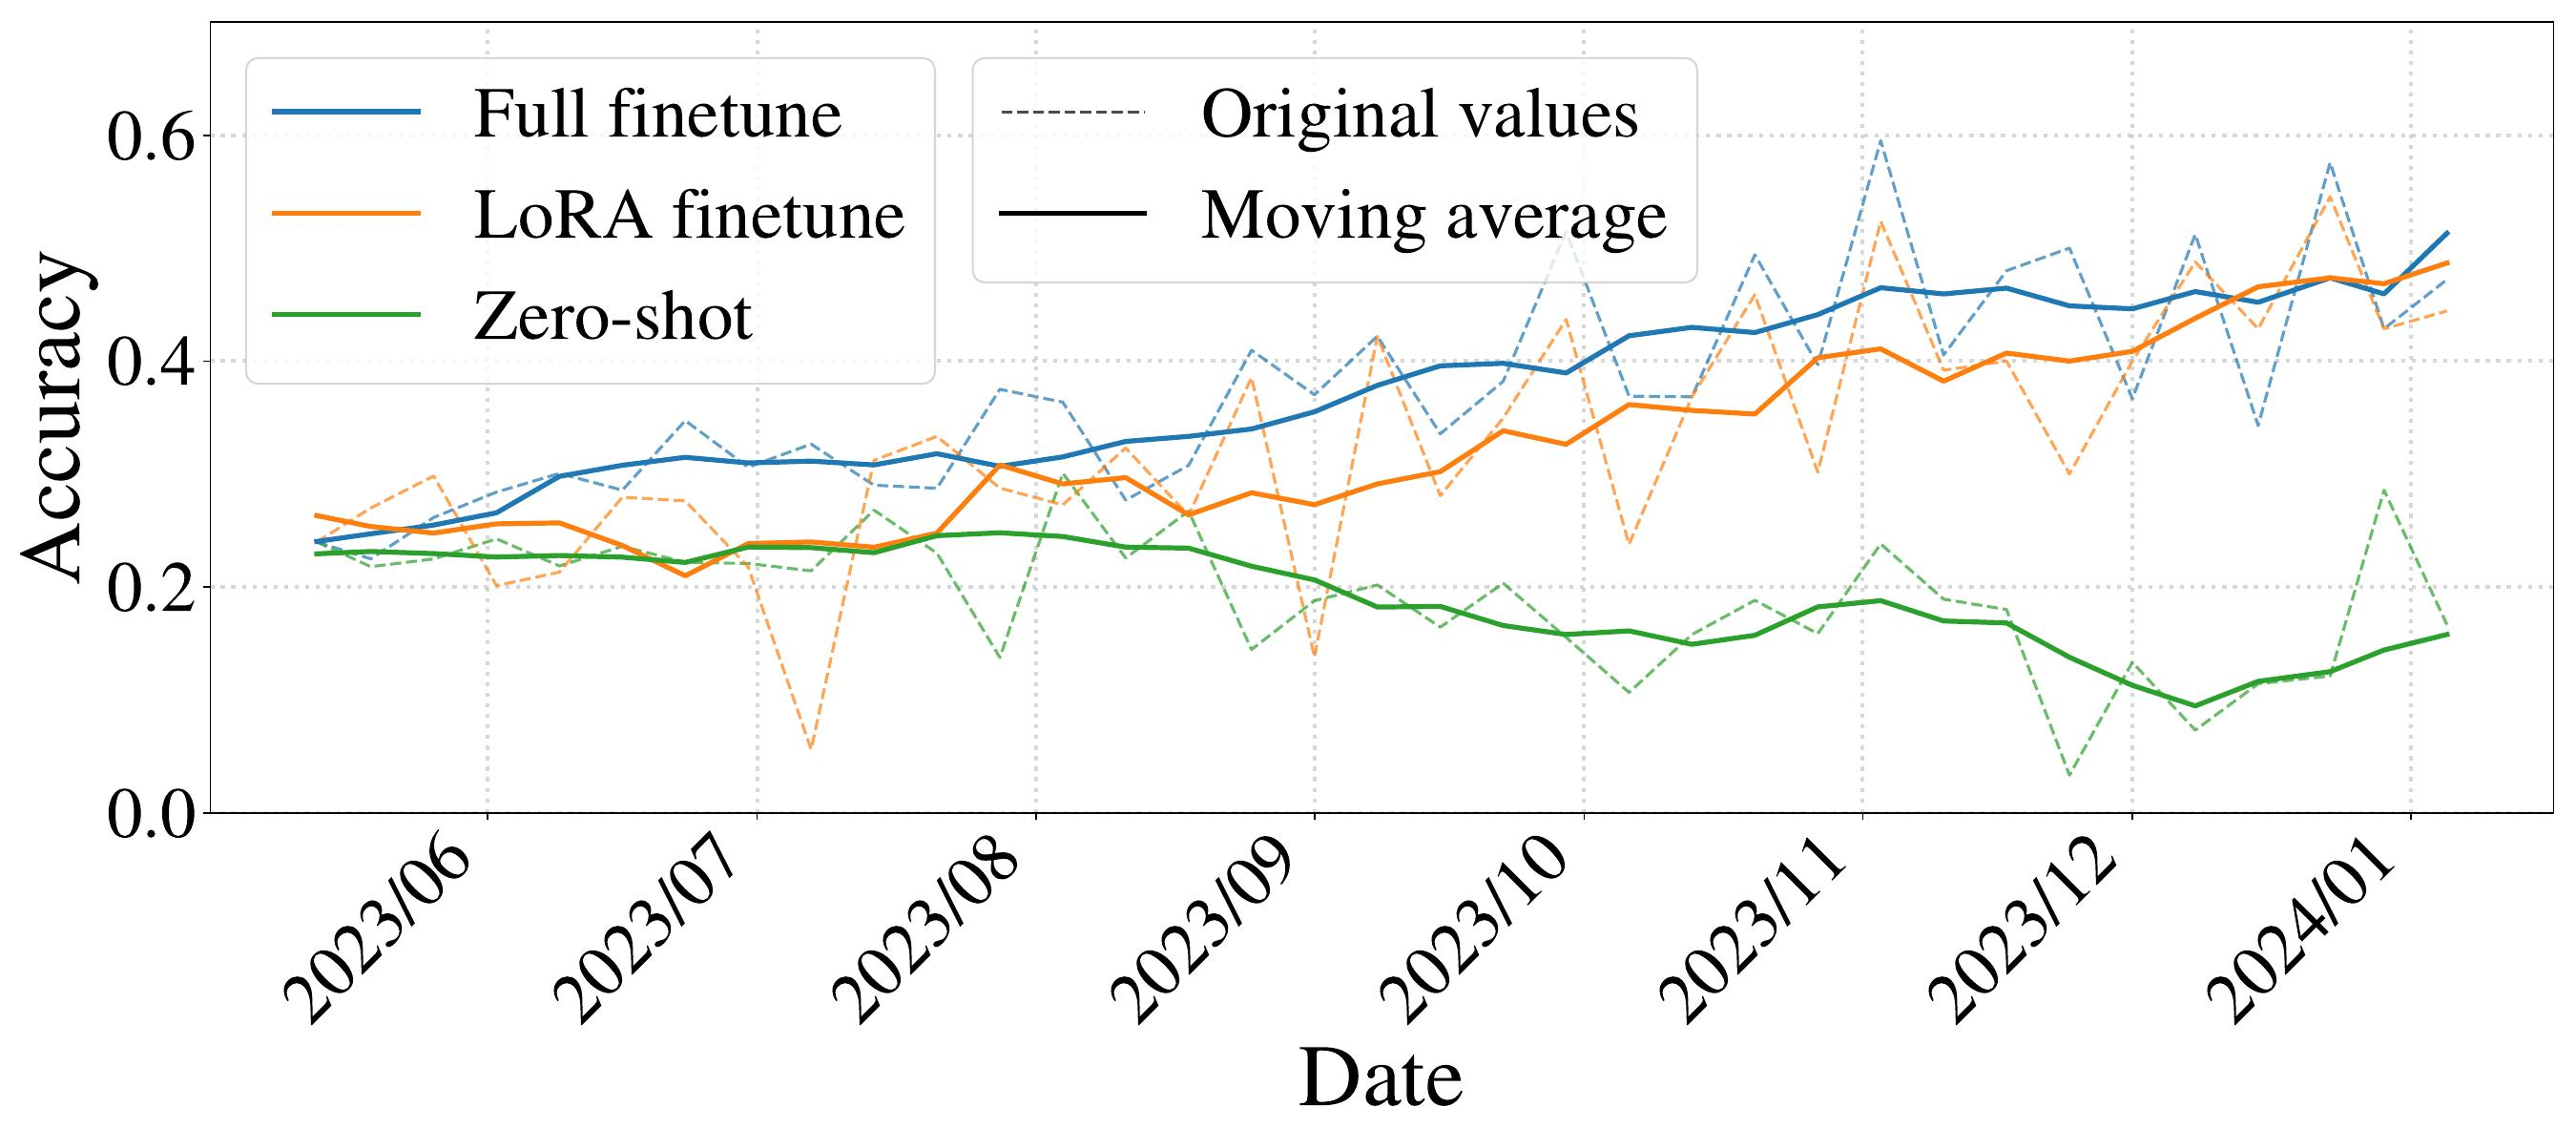
\includegraphics[width=0.7\textwidth]{all_data_1_35_with_legend.jpg}
  \caption{Incremental accuracy over time on all users: zero-shot, full fine-tuning and LoRA fine-tuning (dashed: weekly values; solid: volume-weighted moving average).}
  \label{fig:all}
\end{figure*}
Figure~\ref{fig:all} shows weekly accuracy and the moving average. Read from the plot, the zero-shot model starts near 0.23 and ends near 0.16 in the smoothed curve, i.e., it does not benefit from the passing time and drifts slightly downward over the plotted period. With fine-tuning on accumulated logs, the smoothed accuracy of both full fine-tuning and LoRA rises from roughly 0.24--0.26 to about 0.51 and 0.49, a gain of roughly 25 percentage points over their own starting values and about 33--35 points above the zero-shot curve at the end. Full fine-tuning is above LoRA for most of the period and the two nearly meet near the end of the plot. The weekly (dashed) values fluctuate by more than ten points from week to week, which is why the weighted moving average is part of the protocol; individual weekly differences between methods should not be interpreted.

\begin{figure}[t]
  \centering
  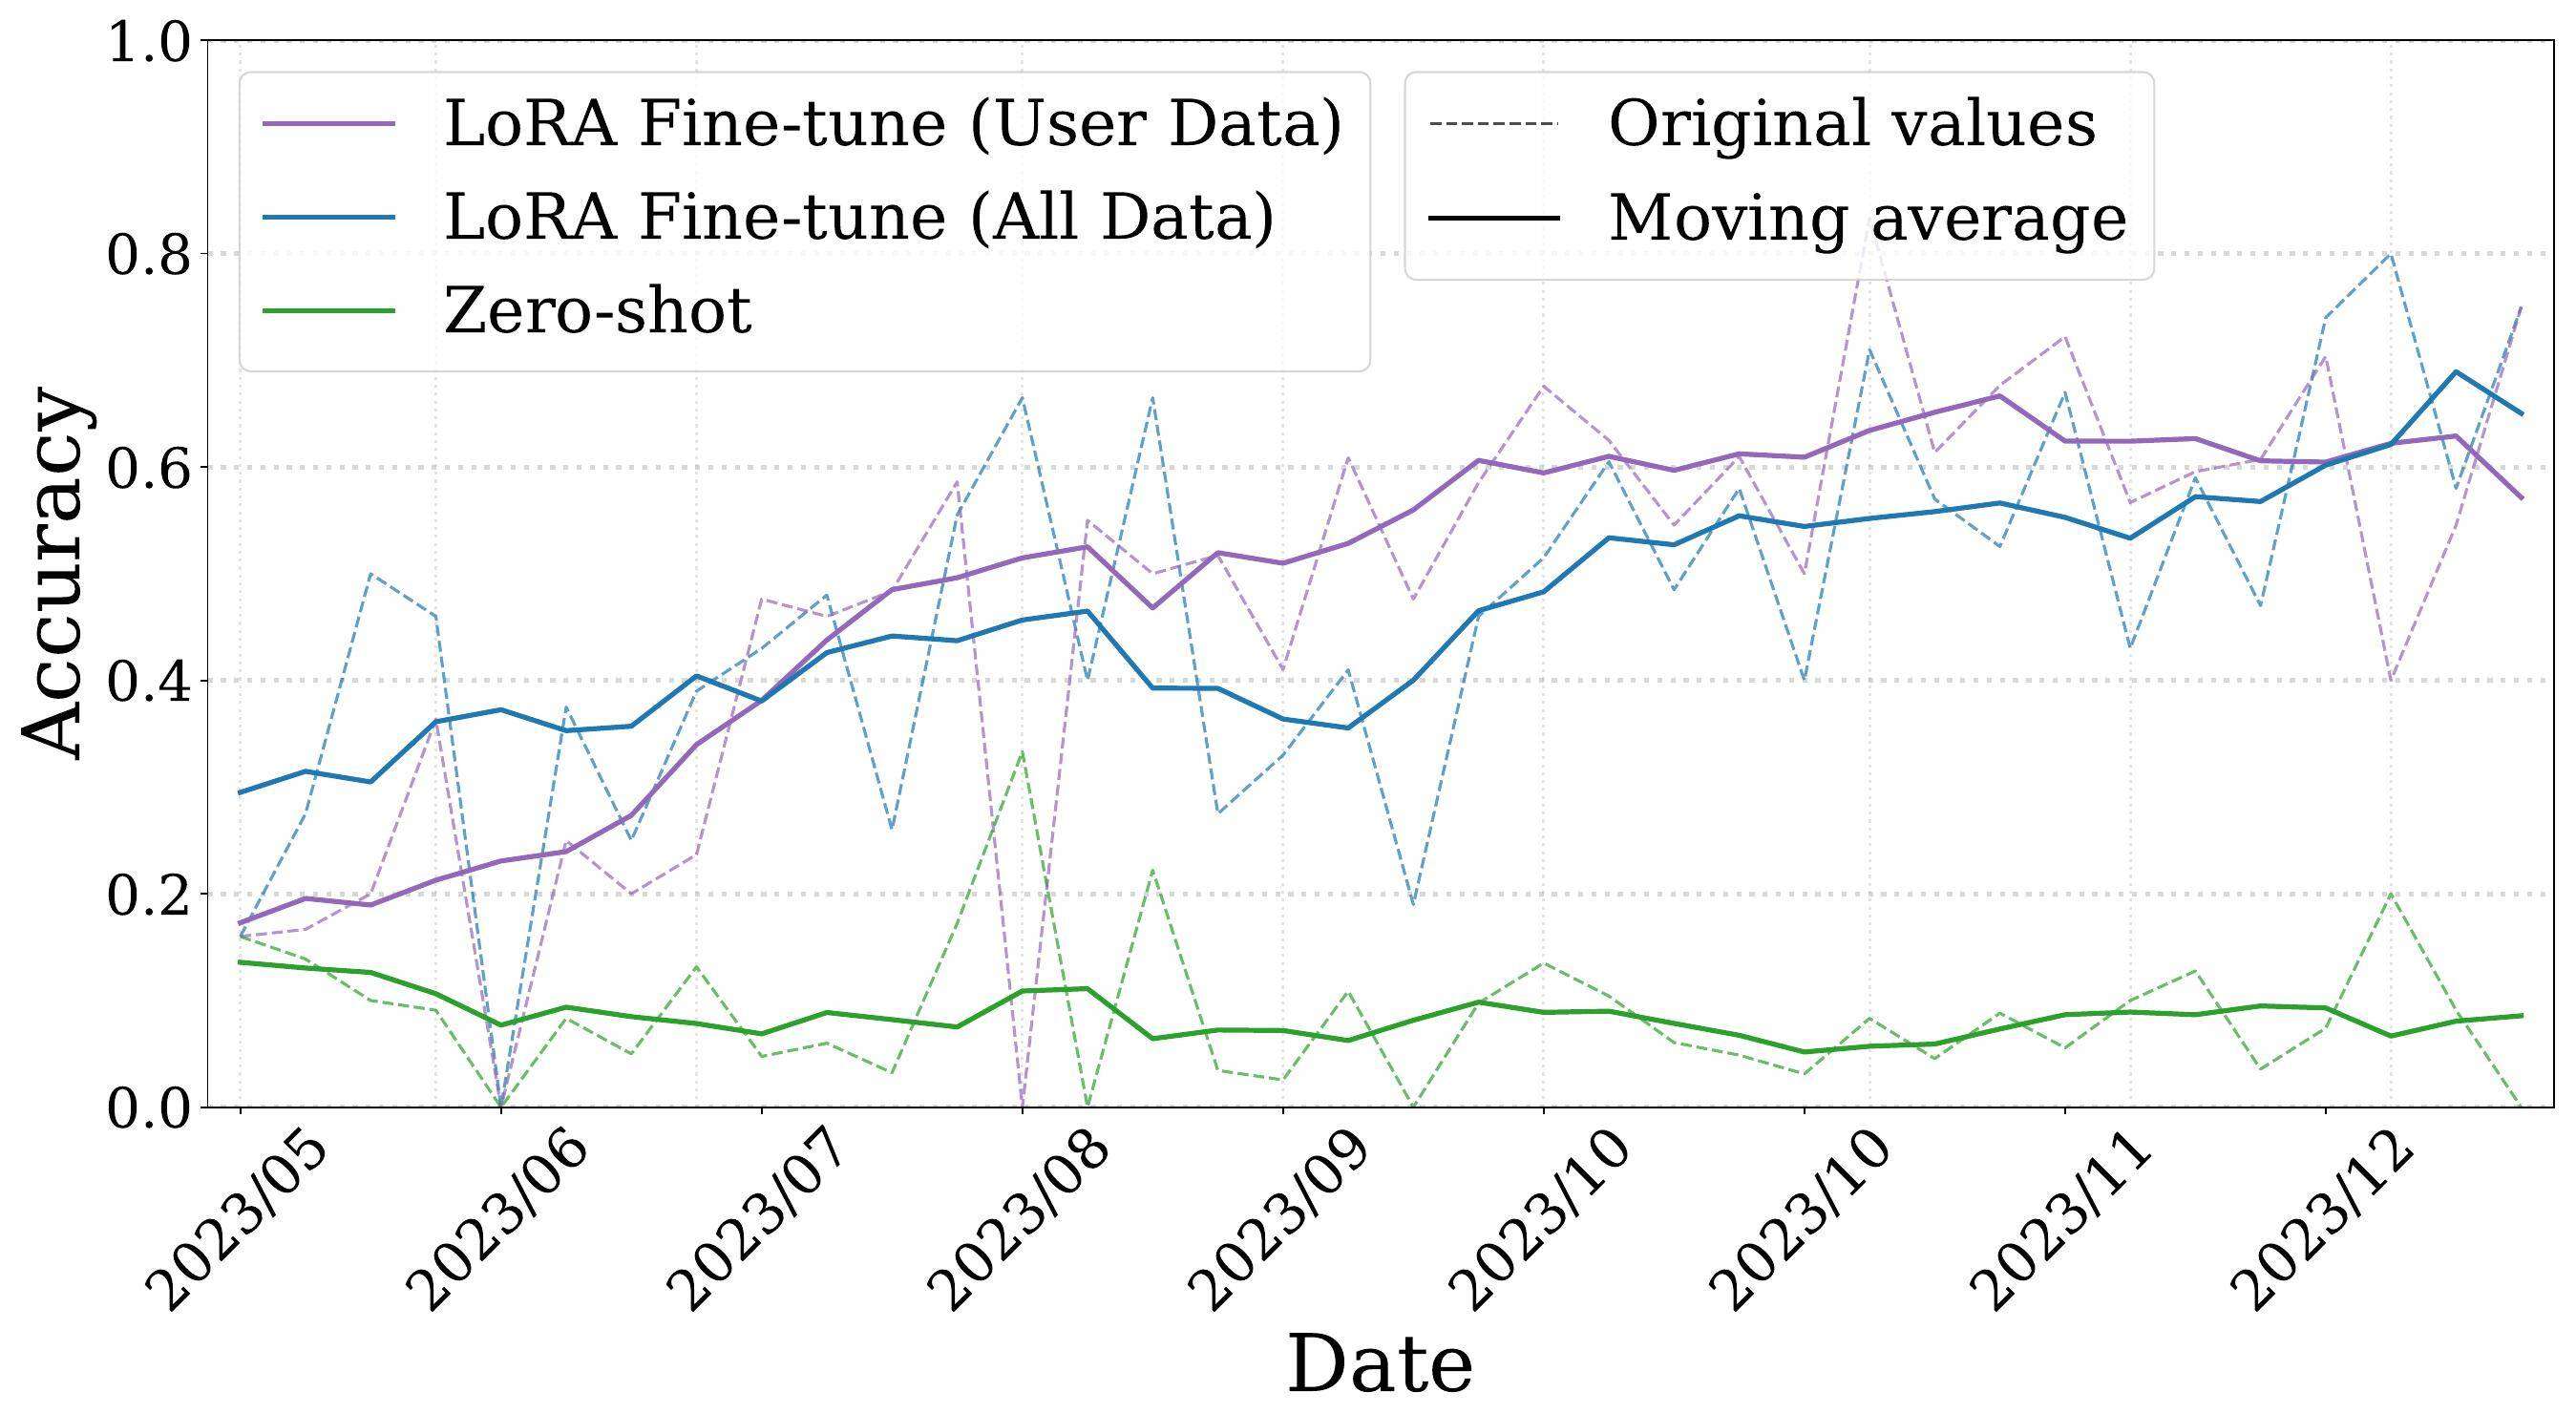
\includegraphics[width=0.9\columnwidth]{user_zero_lora_ma_wide_legend.jpg}
  \caption{Accuracy over time for User A: zero-shot, LoRA fine-tuned on all users' data, and LoRA fine-tuned on User A's data only (dashed: weekly; solid: moving average).}
  \label{fig:usera}
\end{figure}
Figure~\ref{fig:usera} focuses on a heavy logger (User A). Zero-shot accuracy stays around 0.1 (about 0.14 at the start and 0.09 at the end of the smoothed curve). LoRA fine-tuning on this user's data increases from about 0.17 to roughly 0.6, a gain of roughly 40--50 percentage points, and is higher than the all-users model from about July until about early December (for example roughly 0.60 versus 0.55 in October). The comparison is not uniformly in favour of personalization: the all-users model is better early, when the user has little data (about 0.3 versus 0.17 at the start), and it is again above the user-specific model in the final weeks of the plot (about 0.65 versus 0.57). We therefore conclude that user-specific adaptation can match or exceed adaptation on all users once enough personal history exists, but our evidence comes from one user and does not show that it always overtakes it.

\subsection{Task 3: menu-aware classification}
\begin{figure}[t]
  \centering
  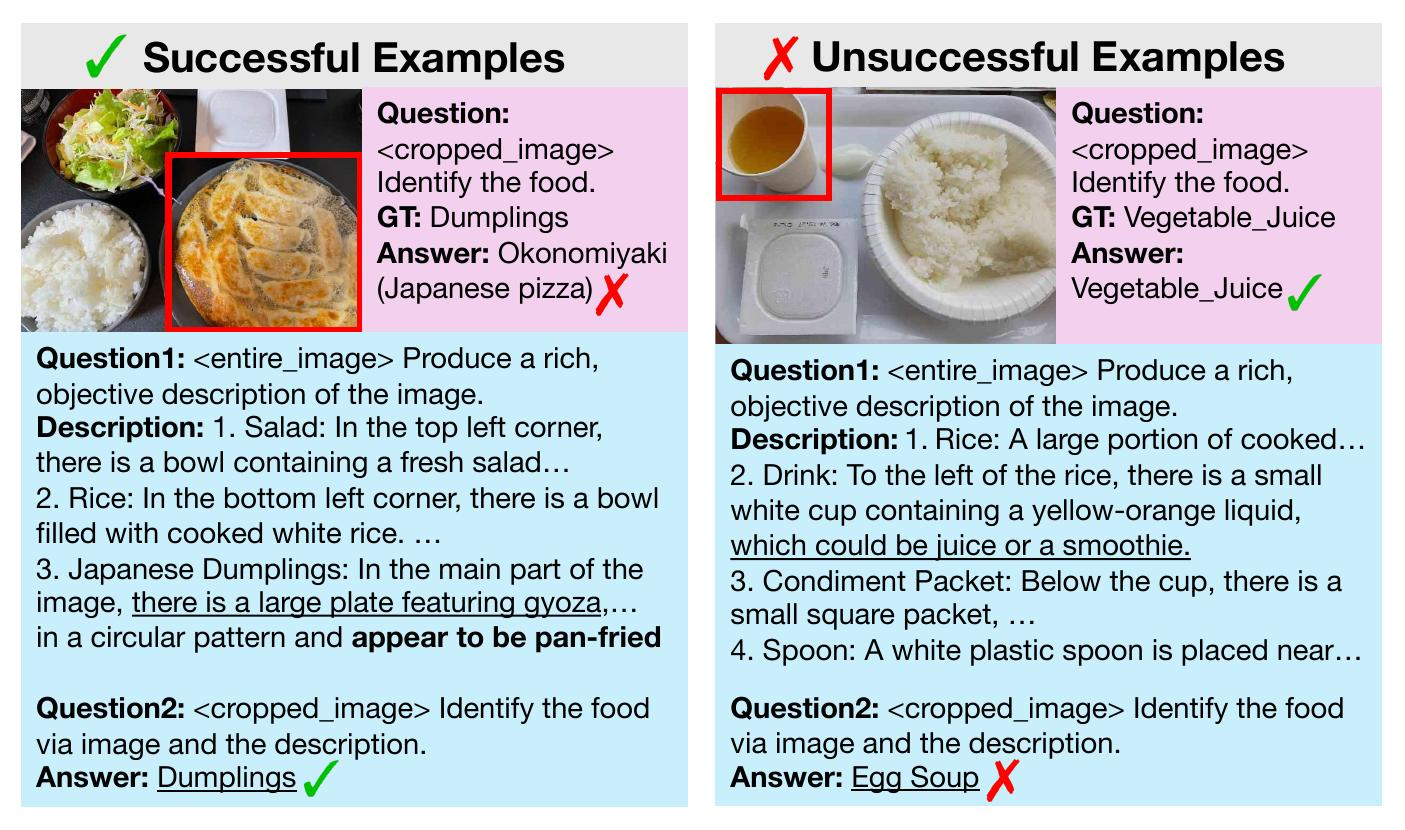
\includegraphics[width=0.9\columnwidth]{description_eg.jpg}
  \caption{Examples of description-guided classification: a case in which the description corrects the answer (left, dumplings) and a case in which it introduces an error (right, vegetable juice becomes egg soup).}
  \label{fig:desc}
\end{figure}
\begin{table}[tb]
  \centering
  \caption{Task~3 (menu-aware classification of dishes in multi-dish images) with a Qwen-VL-7B-Instruct model: F1, Precision@1 and Recall@$K$ without and with a menu-level description of the whole image. The description raises F1 and P@1 but lowers all recall values; $\Delta$ is with minus without description. \textbf{Bold}: better of the two rows.}
  \resizebox{\columnwidth}{!}{\begin{tabular}{@{}lccccc@{}}
    \toprule
    & \textbf{F1}~$\uparrow$ & \textbf{P@1}~$\uparrow$ & \textbf{R@1}~$\uparrow$ & \textbf{R@3}~$\uparrow$ & \textbf{R@5}~$\uparrow$ \\
    \midrule
    w/o description & 0.1594 & 0.1019 & \textbf{0.3656} & \textbf{0.4590} & \textbf{0.4781} \\
    w/ description  & \textbf{0.2304} & \textbf{0.1788} & 0.3240 & 0.4032 & 0.4336 \\
    \midrule
    $\Delta$        & $+$0.0710 & $+$0.0769 & $-$0.0416 & $-$0.0558 & $-$0.0445 \\
    \bottomrule
  \end{tabular}}
  \label{table:desc_guided}
\end{table}

Table~\ref{table:desc_guided} shows that supplying a whole-meal description raises F1 from 0.159 to 0.230 and P@1 from 0.102 to 0.179, while R@1 falls from 0.366 to 0.324 and R@3 and R@5 also fall (0.459$\to$0.403, 0.478$\to$0.434). According to the experiment log summarized in the study overview, the description corrected 687 errors and caused 1,222 new ones, a net loss of 535 predictions, consistent in direction with the R@1 drop; we could not recompute these counts from the tables. Figure~\ref{fig:desc} illustrates both outcomes: a description that mentions gyoza turns a wrong answer into ``Dumplings'', whereas a description that hedges between juice and a smoothie, together with other items in the scene, leads to a wrong ``Egg Soup''. Context is thus not a free improvement: it shifts the precision--recall balance, and the preferable direction depends on how the application uses the output. We tested no other way of providing context, and this is a single run of one model.

\section{Discussion}
\paragraph{What the benchmark measures.} FoodLogAthl-218 measures recognition of logged dishes under natural frequency, casual imaging and multi-dish meals, and the ability of models to improve with a user's accumulating records. The results show that current systems are far from reliable on this data, that model ranking is metric-dependent, and that adaptation along time and meal context change outcomes substantially. 

\paragraph{What it does not measure, and limitations.} (1) All data come from one application and its users, which is likely concentrated in one country and food culture (the application and the example images are Japanese); the cuisine label ``International'' in Table~\ref{Food image dataset table} should not be read as a claim of balanced global coverage. (2) Labels derive from user-submitted logs and application proposals, followed by manual correction and automated consolidation with GPT-4o; inter-annotator agreement was not measured, so residual label noise and the subjectivity of class merging are not quantified. (3) CLIP-based outlier filtering and the minimum of ten samples shape the label space and probably remove unusual but valid samples; the benchmark therefore represents a filtered view of the logs. (4) The LMM protocol relies on a text embedding model to map free-form output to labels, which adds error unrelated to vision. (5) Results are single runs without confidence intervals; the Task~2 and Task~3 findings rest on one model family, and the personalization finding on one user. (6) The diversity statistics are descriptive, and the benchmark measures neither nutritional estimation nor portion size. (7) The images come from private logs rather than public web pages, which should limit overlap with the pre-training data of the evaluated models, but we did not test for leakage. Users should therefore treat the benchmark as a realism-oriented evaluation set to complement, not replace, curated benchmarks.

\section{Conclusion}
We introduced FoodLogAthl-218, a food image benchmark built from real dietary application logs, with 6,925 images, 14,349 dish boxes and 218 classes, and three tasks covering closed-set, continual user-aware and menu-aware classification. The baselines show that dish recognition under real logging conditions remains difficult (best R@1 0.424, best R@5 0.600), that the ordering of systems depends on the metric, that the dataset is more diverse and less separable than UEC-Food 256, that models benefit from adaptation along the time axis, and that meal descriptions trade recall for precision. The benchmark is intended to let these questions be studied under realistic conditions, within the limitations stated above.

\bibliographystyle{ACM-Reference-Format}

\bibliography{references}

\end{document}
